\subsection{Developers using AdaptUI}
\label{sec:developers}

Before introducing the results obtained from working with potential final users
of AdaptUI (as consumers of adapted user interfaces), an experiment has been
carried out involving developers with previous experience with Android development
and semantics. This experiment aims to evaluate the provided \acp{api} and to 
compare the differences between performing a configuration of the user interface 
in Android and in AdaptUI. 

As AdaptUI provides an \ac{api} divided in two (see Section~\ref{sec:application_layer}), 
this experiment has been fragmented accordingly. The first part of the experiment 
considers the user interface adaptation itself. The adaptation \ac{api} eases the 
adaptation process through methods which modify the aspect of the elements 
displayed on the screen. Section~\ref{sec:adaptation_api} details its most 
significant provided methods. The second part's goal is to show developers how 
to modify the knowledge of the AdaptUIOnt ontology. These methods are listed in 
Section~\ref{sec:knowledge_api}.

\subsubsection{The adaptation \ac{api}}
\label{sec:adaptation_api_experiment}

As mentioned in Section~\ref{sec:adaptation_api}, the adaptation \ac{api} provides 
a set of methods whose purpose is to facilitate the adaptation process for 
developers. The purpose of this part of the experiment is to check developer's 
feedback when dealing with the AdaptUI framework by collecting their opinions.
To do so, the experiment presents an Android application developed with the 
Eclipse\footnote{https://eclipse.org/} \ac{ide}. It includes a layout configuration 
\ac{xml} file with the corresponding declaration of several user interface views
(see Listing~\ref{lst:default_layout}), and also an \textit{onCreate} main method, 
shown in Listing~\ref{lst:default_oncreate} (the default aspect of the application
is illustrated through Figure~\ref{fig:default_layout}). The developers 
participating in this experiment are guided through a brief explanation of the 
available adaptation \ac{api} methods. Once they are aware of the possibilities 
the framework provides, they are asked to modify the aspect of the listed views.

\inputminted[linenos=true, fontsize=\footnotesize, frame=lines]{xml}{5_experiments_and_results/default_layout.xml}
\captionof{listing}{The default layout defining a grid layout, a text view,
a button and an edit text.\label{lst:default_layout}}

\inputminted[linenos=true, fontsize=\footnotesize, frame=lines]{java}{5_experiments_and_results/default_oncreate.java}
\captionof{listing}{The default \textit{onCreate} method.\label{lst:default_oncreate}}

\begin{figure}
\centering
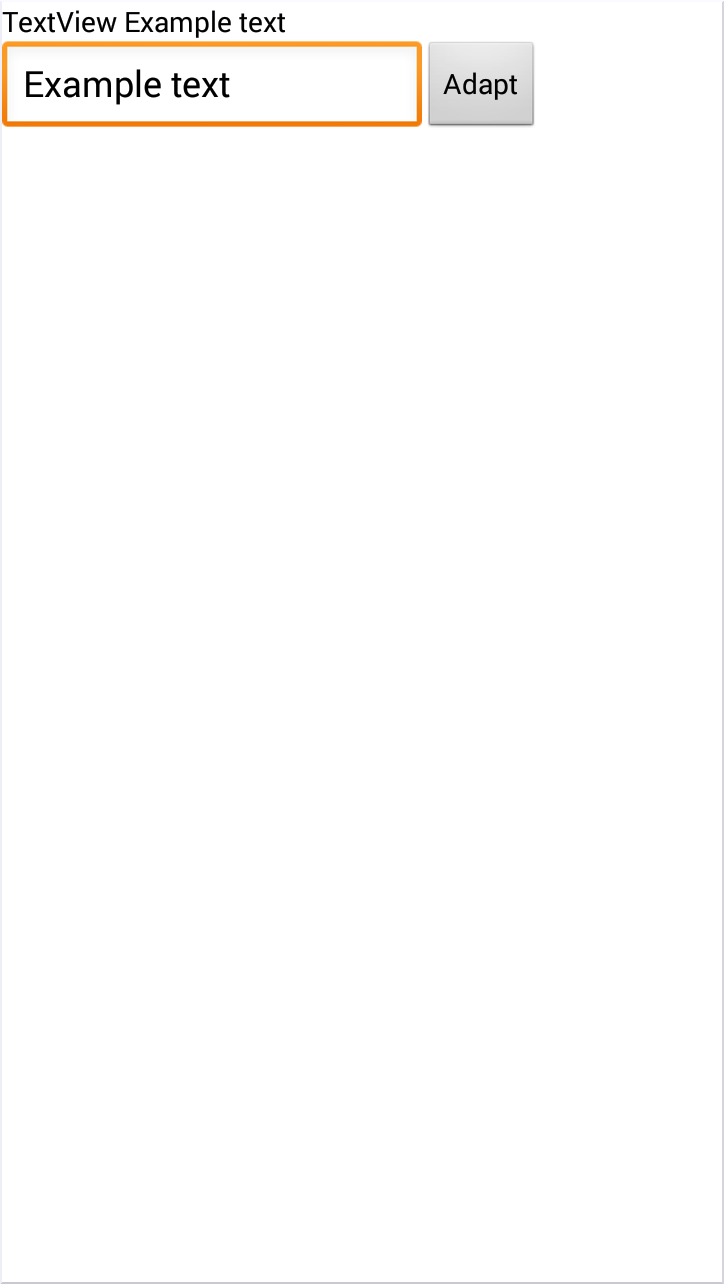
\includegraphics[width=0.25\textwidth]{default_layout.png}
\caption{The corresponding user interface considering the layout specified in
Listing~\ref{lst:default_layout}.}
\label{fig:default_layout}
\end{figure}

Obviously, in order to adapt the application, developers need a copy of the
AdaptUIOnt ontology, in which the corresponding values for the adaptation are
semantically represented. Hence, developers are asked to install the Capabilities 
Collector in their Android devices. Thus, they can add new knowledge to the ontology.

Listing~\ref{lst:default_oncreate} shows the presented \textit{onCreate} method, 
which defines the views listed in Listing~\ref{lst:default_layout}. Using AdaptUI 
developers reach the \textit{onCreate} shown in Listing~\ref{lst:adaptui_oncreate},
which includes the corresponding calls to the provided adaptation \ac{api}.

\inputminted[linenos=true, fontsize=\footnotesize, frame=lines]{java}{5_experiments_and_results/adaptui_oncreate.java}
\captionof{listing}{The AdaptUI \textit{onCreate} method.\label{lst:adaptui_oncreate}}

Thus, the resulting adapted user interface is illustrated by Figure~\ref{fig:adapted_layout}.
While Figure~\ref{fig:default_layout} shows a default disposition and configuration
of the user interface items described in Listing~\ref{lst:default_layout}, in this
case they have been adapted according to Listing~\ref{lst:adaptui_oncreate}.

\begin{figure}
\centering
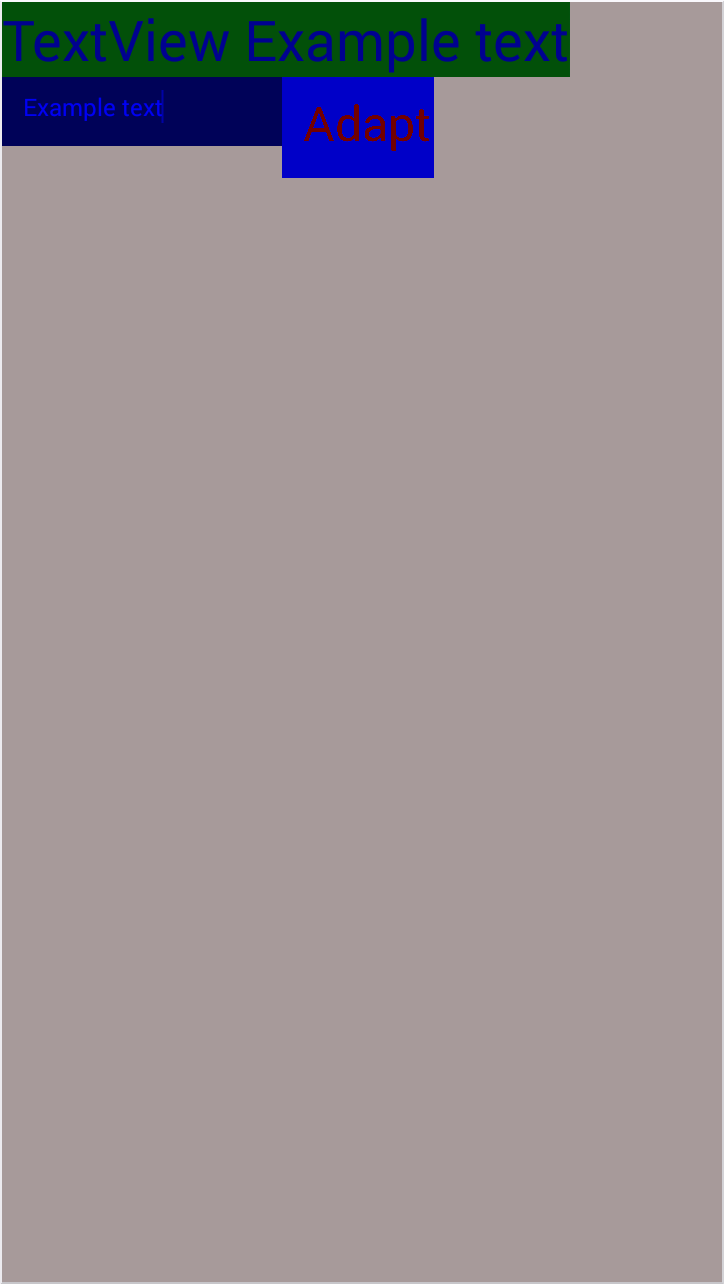
\includegraphics[width=0.25\textwidth]{adapted_layout.png}
\caption{The corresponding user interface considering the layout specified in
Listing~\ref{lst:adaptui_oncreate}.}
\label{fig:adapted_layout}
\end{figure}



\subsubsection{The knowledge editor \ac{api}}
\label{sec:knowledge_api}

The knowledge editor \ac{api} provides a set of methods to modify the knowledge
stored in the ontology. Imported as a library from a Java project, this \ac{api}
allows to add and remove classes, individuals, object and datatype properties,
and rules. In this experiment developers are asked to modify the ontology by
adding new concepts to be used by the adaptation \ac{api}.